\chapter{JavaCard Vulnerability Scanner the JavaCard testing framework}
Naturally, a question arises: Is there even a need for a tool, that would test the shortcomings of JavaCard VM and JavaCard RE?  In the first chapter we have mentioned previous research, some of which include a source code for a POC attack as a part of its results. However, if the reader imagines himself holding a JavaCard and wondering, whether it is vulnerable to a specific kind of an attack there is still \textit{a lot} of work to be done. Some of the POCs are \textit{only} included in the original paper and not accompanied with the source and build files. Or in the case of vulnerabilities discovered by Security Explorations the source code is included (as a ZIP archive), but the attacks are automated only for use with the reference implementation of JCRE. Also, they are built only with SDK 3.0.5GA. Given the number of new attacks discovered in the last years~\cite{se:oracle:part1, se:oracle:part2, se:oracle:part3, se:gemalto:part1, se:gemalto:part2} it is increasingly harder to perform systematic security analysis of a real JavaCard against all known (logical) attacks.


Overall, we believe, that the JavaCard community would benefit from an automated testing framework, that cuts down the time and work required to test a real JavaCard significantly. And so the answer to the question phrased above is: Yes. JavaCard Vulnerability Scanner allows the user to test the integrated attacks  for all SDK versions for which the attack is built. After the user performs the initial setup of the framework (see~\ref{sec:invocation}) she only needs to insert a JavaCard into a smart card reader and invoke the main utility \javus. The results are presented through locally served web pages.

Currently, all the vulnerabilities described with POCs in chapter~\ref{chp:state-of-the-art} are supported by JavaCard Vulnerability Scanner. Further more, some of the vulnerabilities presented in~\cite{sergei} have been manually tested and will be added once they can be build automatically.


% \projectname comes with a command line utility called \javus. Whenever we talk about the complete framework we will use \projectname, but in case we describe the utility we will use \javus.

\section{The design of the testing framework}\label{chp:testing-tool}

% First, we will start with the list of the specifications for the framework. Before we go through them one by one and look at the way that they are implemented in more detail we define some terms and explain the project structure.

% \subsection{The framework specifications}
    We will start by laying down the specifications for the implementation of \projectname:
    \begin{enumerate}
        \item execute registered logical attacks on a real physical JavaCard (see~\ref{sec:build-execute-attacks}),
        \item visualize the results of the attacks in a concise and clear manner (see~\ref{sec:visualization}),
        \item be extensible --- allow adding new attacks in the future (see~\ref{sec:attack-recipe}).
        \item be cross-platform, i.e. support at least Linux and Windows platforms (see~\ref{sec:invocation}),
    \end{enumerate}


    And we also introduce a new terminology, that will be used with few exceptions:

                \begin{enumerate}
                    \item[\textbf{attack}] is the overarching term used for describing a (particular) way of exploiting a vulnerability in JCVM or JCRE\@. Especially, POCs described in previous chapter will be from now on in most cases referred to as attacks,
                        % When we talk about \textbf{a particular} attack we will try to name it as well to avoid confusion. For example, when we say \textbf{ArrayCopy attack} we are talking about the attack exploiting the \mintinline{java}{arrayCopy} method from class \mintinline{python}{javacard.framework.Util} as it is implemented in the directory \filepath{javus/javus/data/attacks/arraycopy},
                    \item[\textbf{stage}] or fully \textbf{an attack stage} is one part of the attack, e.g. the installation of a CAP file, that is required by the attack to work. During another stage we could send an APDU command to a JavaCard. Good example of stages are instructions from the POCs from the chapter~\ref{chp:state-of-the-art},
                    \item[\textbf{scenario}] or fully \textbf{attack scenario} consists of all the stages of an attack, in the source code represented by a python class \mintinline{python}{Scenario}
                    \item[\textbf{run}] describes the execution of a set  of (one or more) attacks on a particular physical JavaCard and is usually referencing the \javusrun command, the expressions \textit{test run, analysis run} etc. are simply synonyms.
                \end{enumerate}

        \subsection{The repository structure}
The project is using Git for its version control and it is mainly a Python package. The following paths are relative from the directory \projectroot, which is the root of the Git repository. The Python sources are in \filepath{javus/}, the attacks' source codes are in \filepath{javus/data/attacks/<attack-name>} in respective directories. The file \filepath{javus/data/registry.ini} defines which attacks are enabled. The main command line utility is called \javus. Full Git repository description is in Appendix~\ref{sec:gitrepo}.


        Now that the reader is familiar with the framework specifications and has overview of the project hierarchy we can go deeper into the internals of the tool. Because the framework takes the advantage of several different tools and integrates them together it was not helpful to follow one particular design pattern. The project is implemented mainly in Python and as such uses the Object Oriented Programming paradigms and also takes the advantage of Python's feature of dynamic imports. Several external tools are used through a \textit{wrapper} class objects, that create internal API (see Appendix~\ref{subsubsec:gpp}).


    \section{Building and executing the attacks}\label{sec:build-execute-attacks}

    The diagram~\ref{fig:full-design-diagram} shows a single run of the testing tool. The blue boxes represent a user input. The user is only required to insert the JavaCard and execute a single command \javusrun (which invokes the \mintinline{bash}{javus.analyzer.App} class, that is responsible for orchestrating the complete analysis). Once the tool is invoked, it loads the registered attacks and executes them one by one. The results are being updated to the database continuously, because the card can stop working any time during the run (as the reader will see in the chapter~\ref{chp:results}).


    Executing multiple attacks automatically is not\linebreak straightforward. For reasons that are explained later in~\ref{sec:uniq-aid} we need to have the ability to dynamically rebuild an attack during the run of the framework. Moreover, the way attack applets and packages are built can differ across the spectrum of attacks.

    \begin{figure}[htb!]
        \centering
        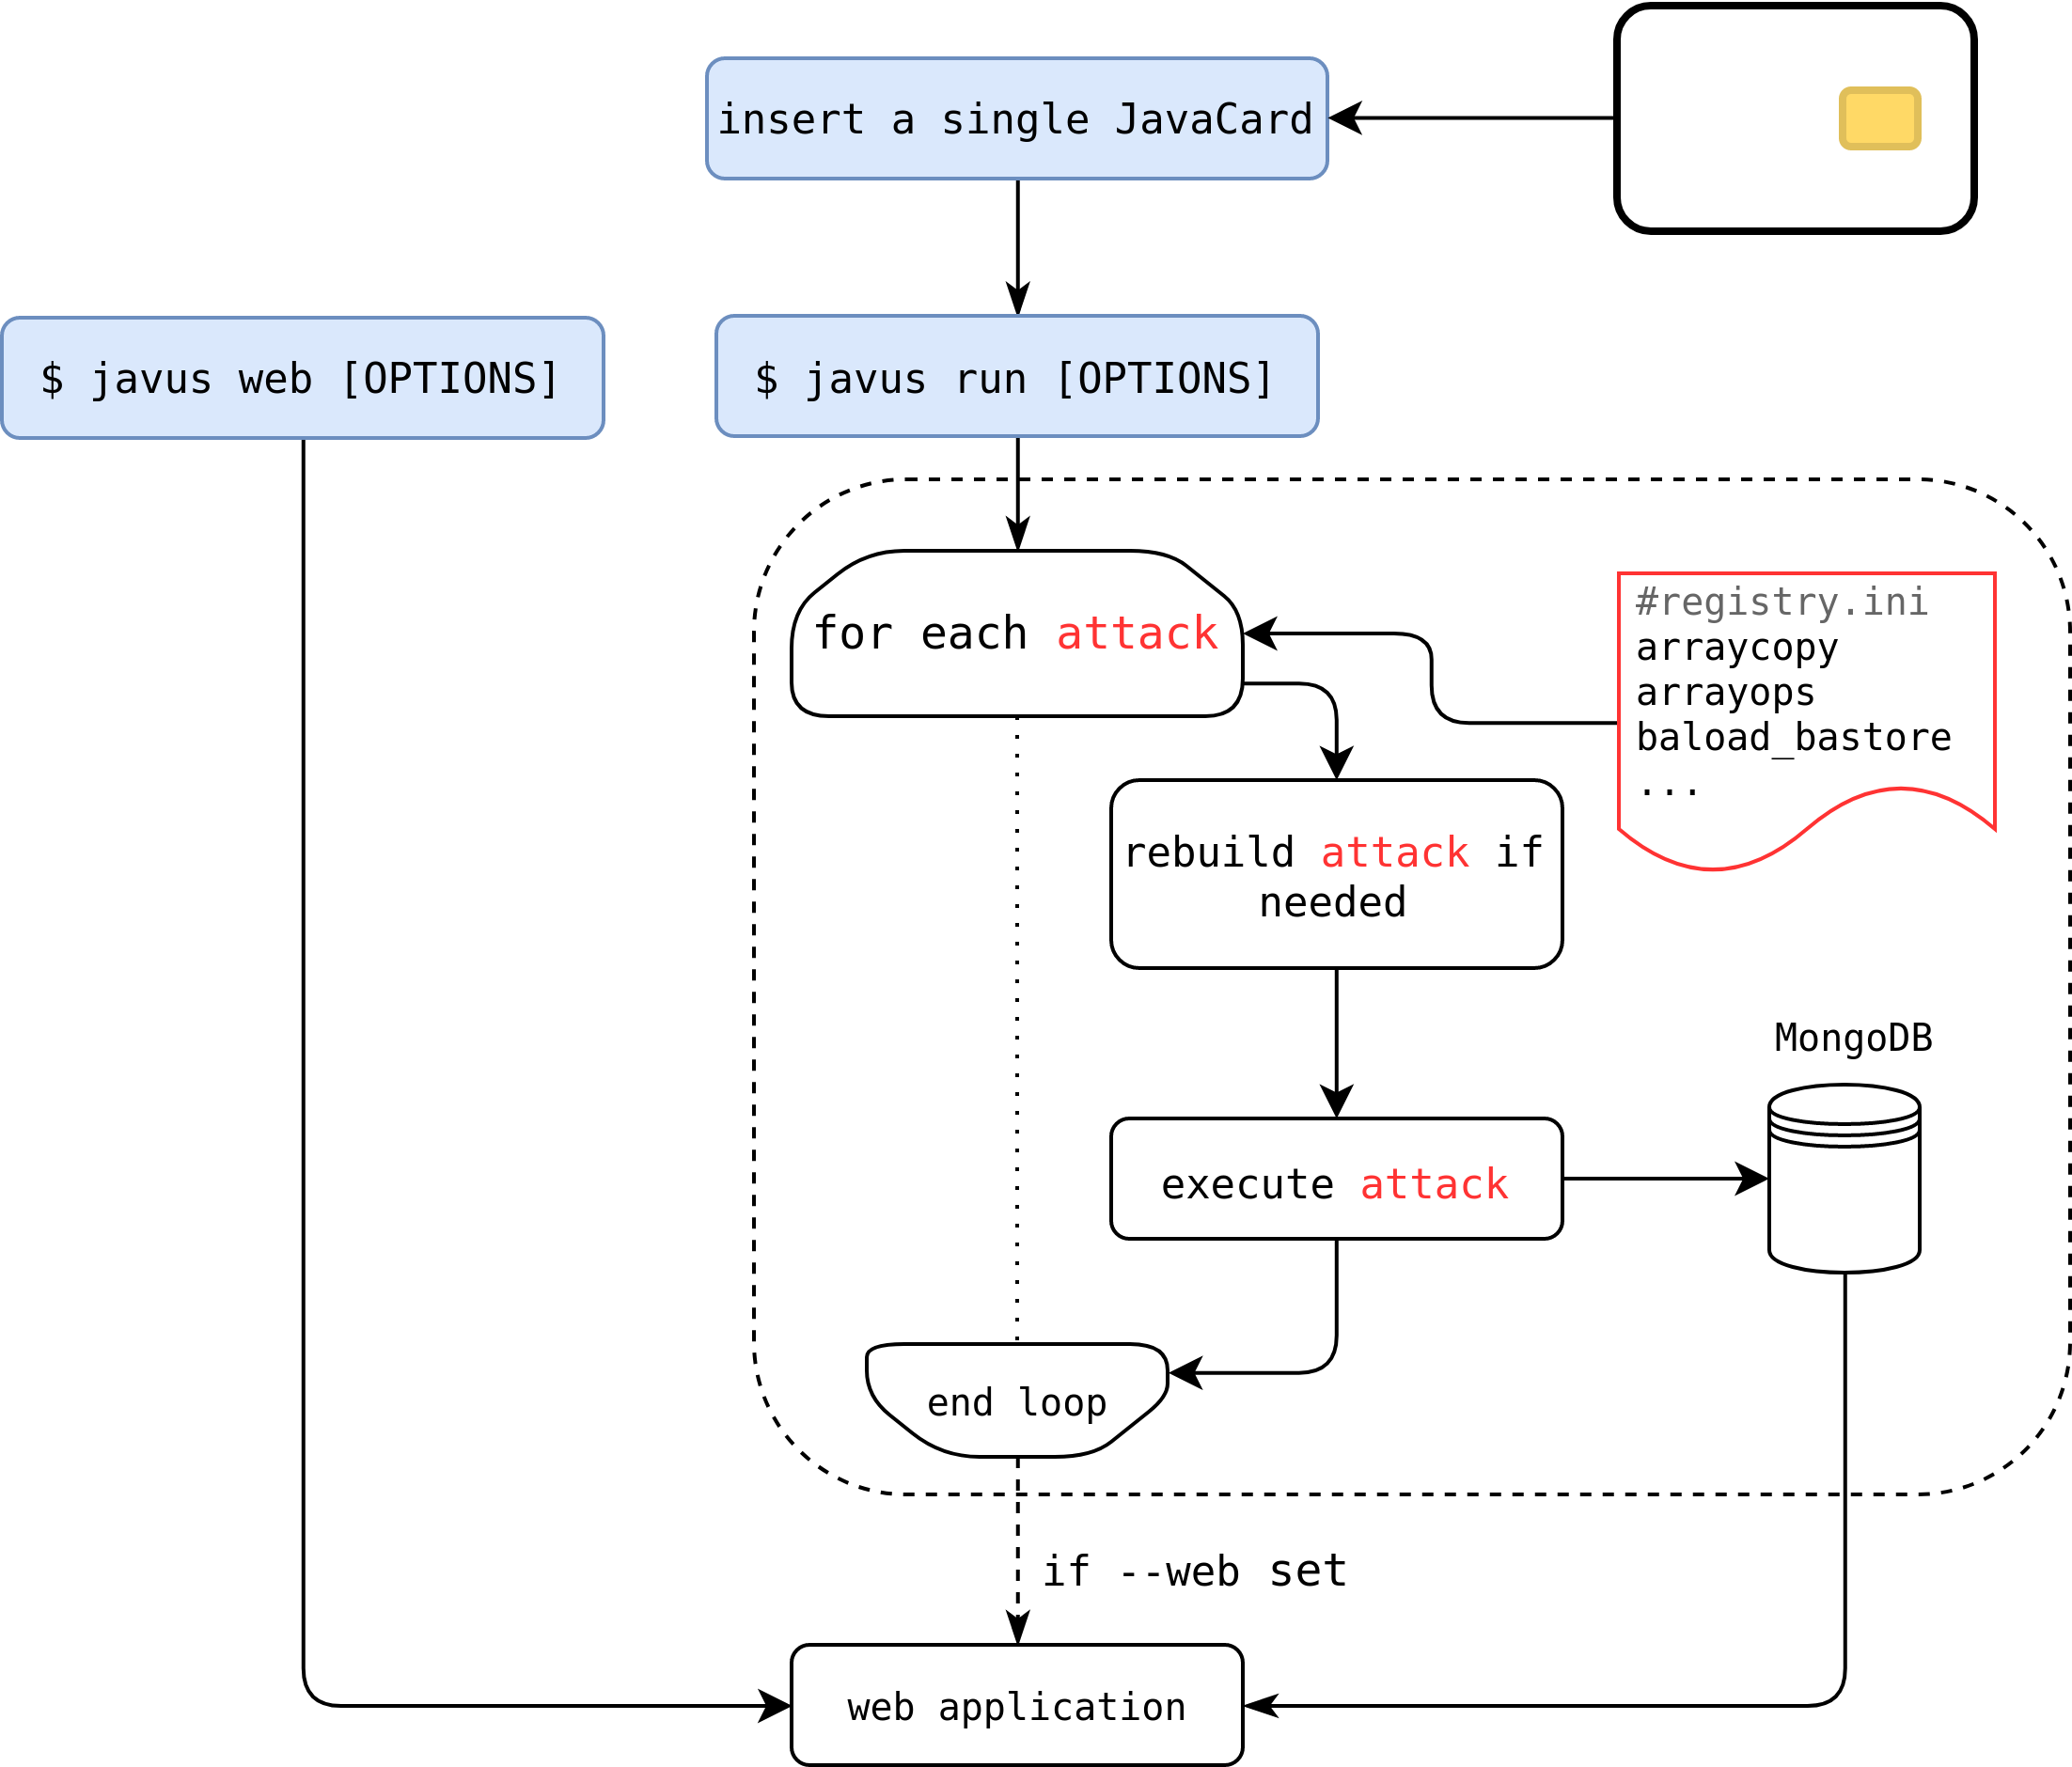
\includegraphics[width=.9\textwidth]{src/diagrams/full-design-new.png}
        \caption{High-level diagram of the run of the application. The part with the dashed rectangle is visualized in more detail in the figure~\ref{fig:execute-attack-diagram}.}
        \label{fig:full-design-diagram}
    \end{figure}

        
    Not only the build process can differ with each attack, but also the execution --- naturaly, each attack can consist of multiple stages (e.g. installing different number of CAP files, sending various number of APDUs). We will cover this in more detail in~\ref{sec:attack-recipe}, but for now, we will only explain, how per attack build and execution is implemented.

    After \shortappclass handles the command line arguments it hands the execution over to \mintinline{python}{javus.analyzer.AnalysisManager}, which iterates over the registered attacks (loaded from \filepath{registry.ini}). For each attack \mintinline{python}{AnalysisManager} loads the appropriate subclass of \shortbuilderclass respectively \shortexecutorclass that is responsible for building, respectively executing the attack. Now we will take a closer look at those two classes. While reading the next sections the reader can consult the diagram in the figure~\ref{fig:execute-attack-diagram}.

    % TODO second diagram, change to <attack>
    \begin{figure}[htb]
        \centering
        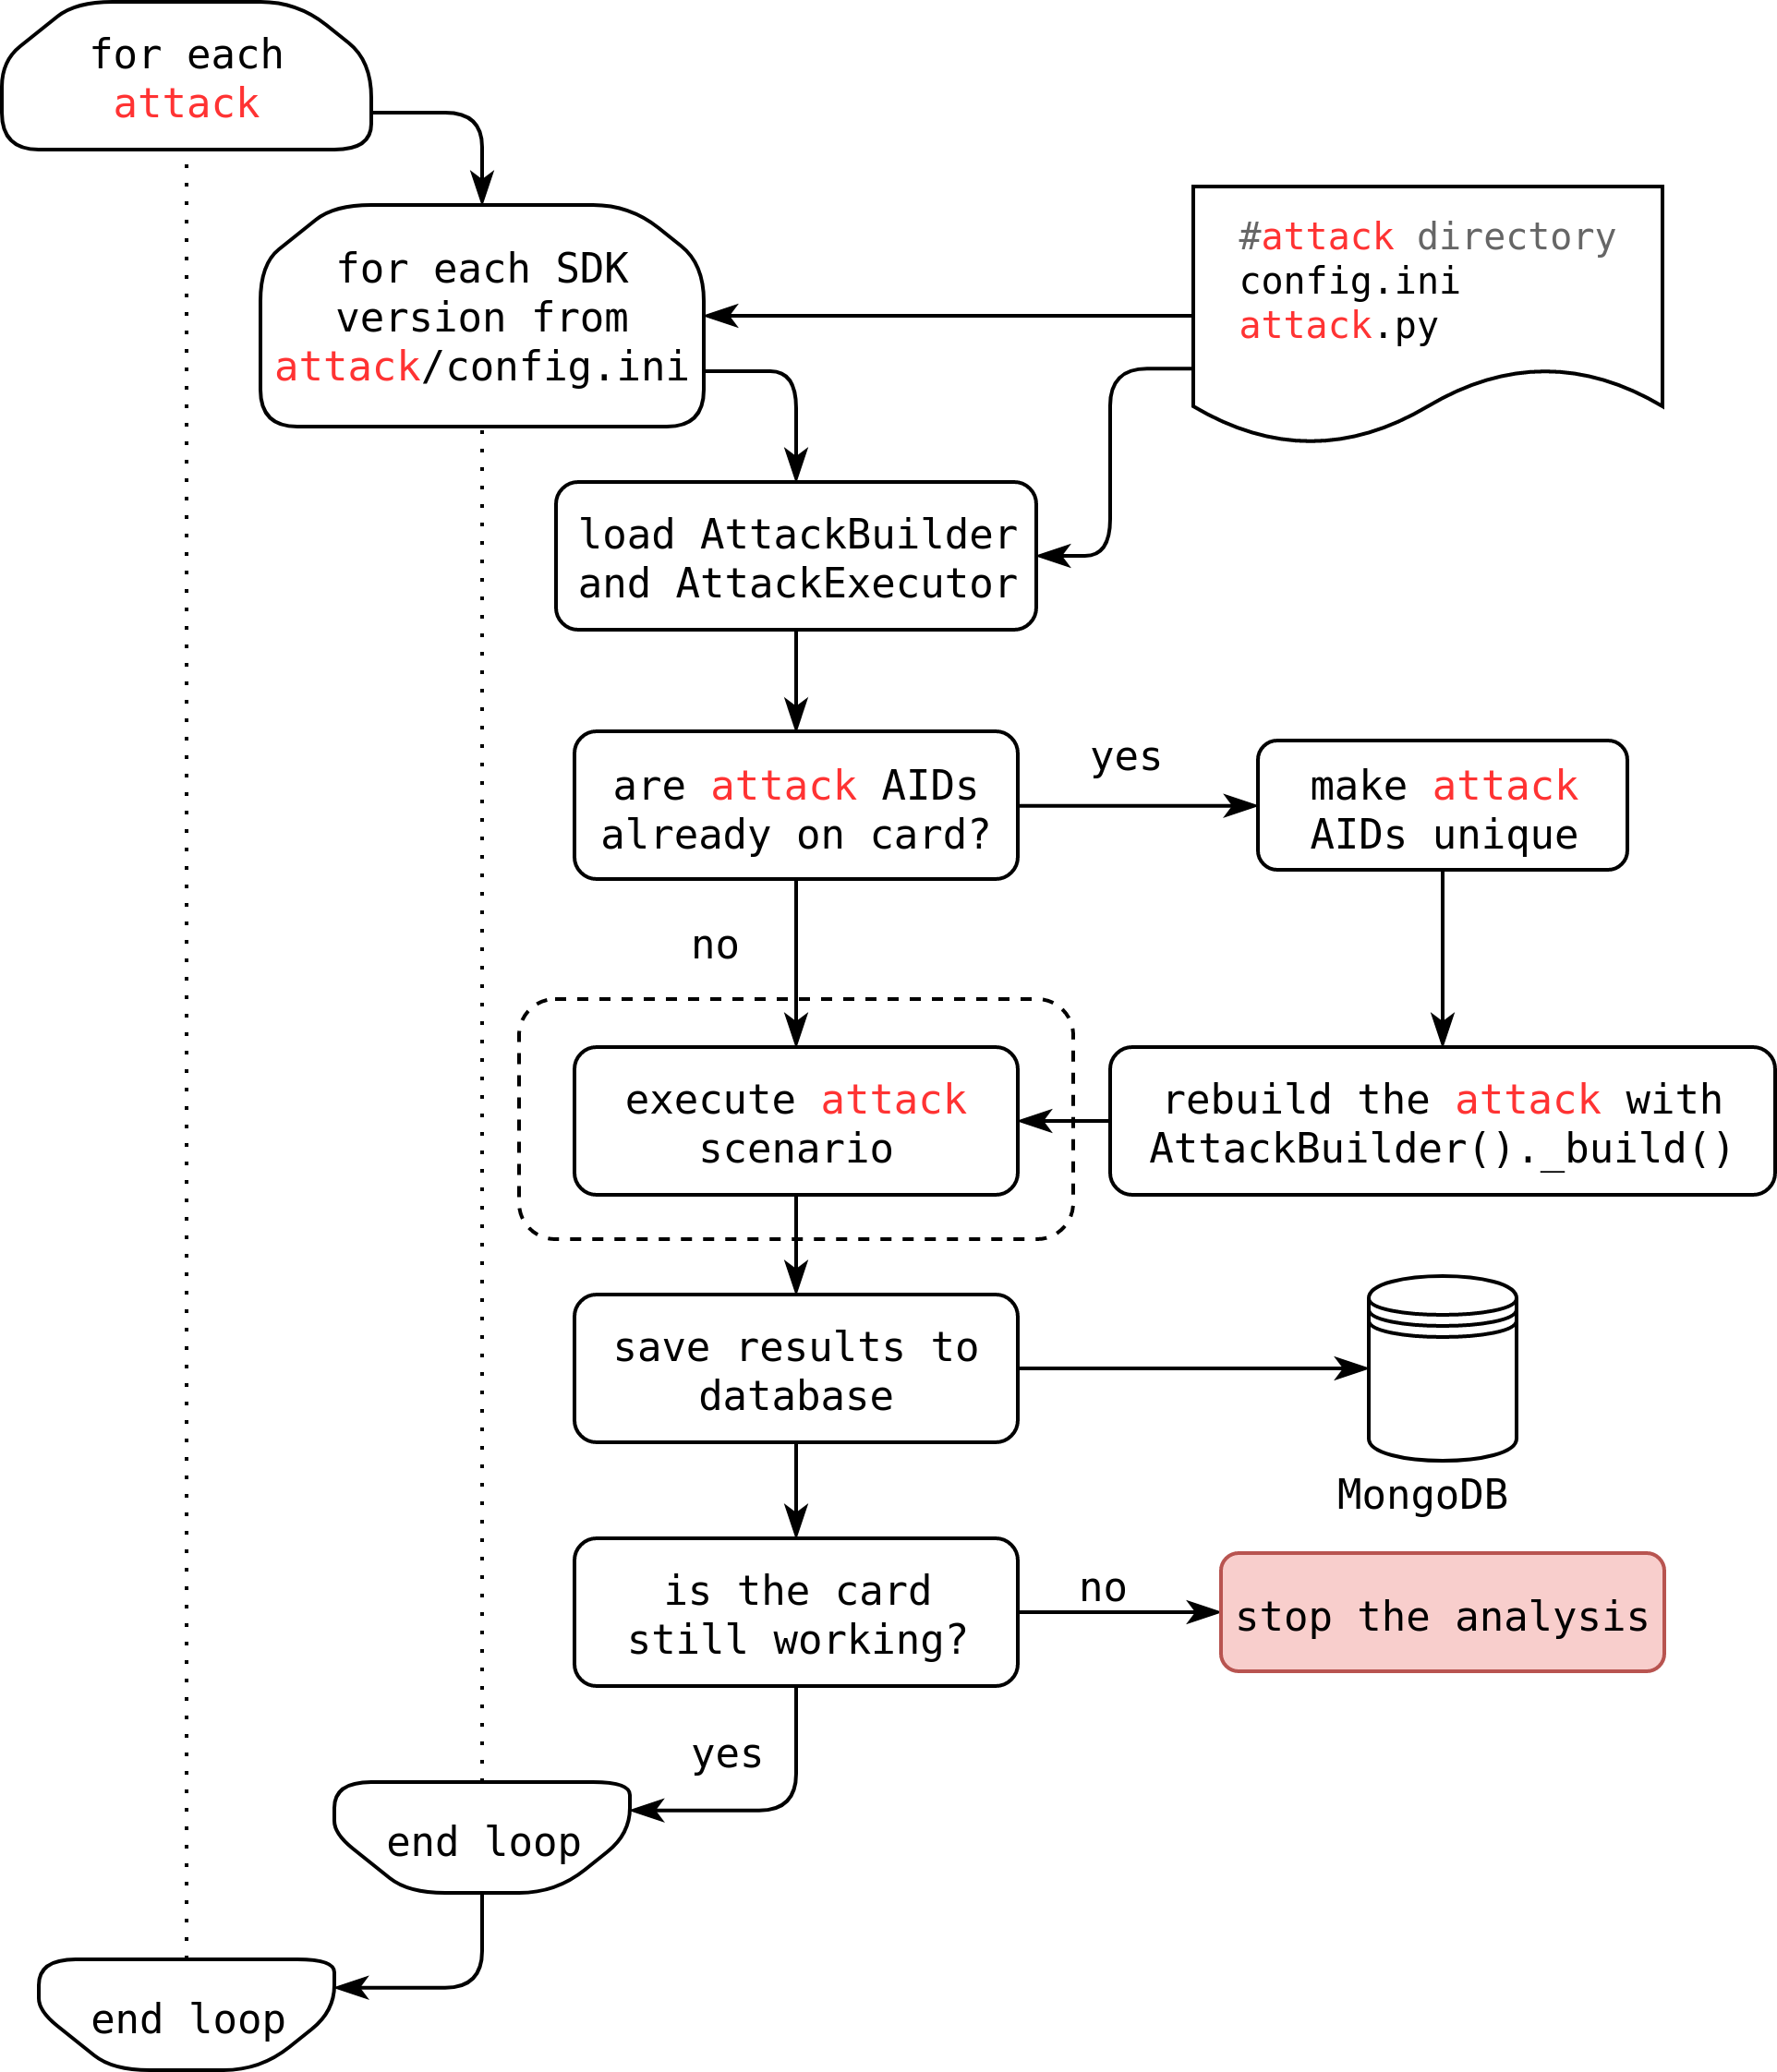
\includegraphics[width=.8\textwidth]{src/diagrams/execute-attack.png}
        \caption{A detailed look at the main attacks execution loop. The final diagram, that fully explains the part in the dashed rectangle is in~\ref{fig:execute-scenario}.}
        \label{fig:execute-attack-diagram}
    \end{figure}



        \subsection{The class \builderclass}\label{subsec:builder-class}
        The ability to build an attack during the run of the analysis means having an automated way of creating all the necessary CAP files, that need to be installed during the attack. Not only creating them but, if the attack requires, also performing any malicious alterations of  e.g.\ the byte code of a particular CAP file (such alteration is necessary for most of the attacks registered in the framework at the moment of writing). Dynamic rebuild of an attack is mainly motivated by the problem of AID uniqueness. In short, an attack would fail before it even started, if any of the AID it was built with is already present on the card (we go into further details in~\ref{sec:uniq-aid}).

        On one hand, attacks naturaly have different build processes (e.g.\ they consists of a different number of packages and applets). On the other hand, some of them might be so similar, that it makes sense for them to share the build process. To allow both we have decided to do the following.
        % To achieve both of those goals, i.e. have the ability to automate the builds while leaving enough room for future attacks, we have decided to do the following.

        To build the CAP files we use Apache Ant. Each attack needs to implement \mintinline{bash}{build.xml} file with a few Ant targets (\ref{subsubsec:ant-targets} discusses the details). The framework provides a class \builderclass, that calls the necesary Ant targets during the runtime. In case a further alteration to the build process is needed the class \shortbuilderclass can be subclassed with the class \attackbuilder and the \mintinline{python}{_build} method can be overridden. If only a single attack needs these changes, it is best to put the implementation of \attackbuilder to \filepath{javus/data/attacks/<attack-name>/<attack-name>.py} (the name of the attack directory and the Python module need to match).
        If, however, the build process is shared by multiple attacks, then the implementation can be added to \filepath{javus/data/attacks/<common-name>.py} (the name can be arbitrary). For the latter case to work it's needed to also add the key value pair \mintinline{ini}{module = <common-name>} to the respective section in \filepath{registry.ini}. There are no real requirements regarding the implementation of \mintinline[breakafter=.]{python}{_build} method. For example, the Security Exploration attacks have a custom Java tool, that is called inside the \mintinline{python}{_build} method (see the file \filepath{javus/data/attacks/security_explorations.py} or~\ref{app:sec:sebuilder} for details).

        The last thing we will mention here is, that each attack can also parametrized by JavaCard SDK version (loaded from \filepath{javus/data/attacks/<attack-name>/config.ini}), that means it can built and executed for several SDKs. As the reader will see in the last chapter, the results differ with SDK version significantly.

        \subsection{The class \executorclass}\label{subsec:executor:class}
            For the execution of a single attack scenario we have implemented the class \mintinline{bash}{BaseAttackExecutor}. This class loads the attack scenario (which is defined simply as \scenario class) during the runtime of the analysis and then executes each stage one by one. The scenario stages are defined as a class level attribute \mintinline{python}{Scenario.STAGES}.

            The class \scenario is loaded from \filepath{javus/data/attacks/<attack-name>/<attack-name>.py} module. For most attacks the scenario needs the same type of stages --- they need to install CAP file(s), send some APDUs and uninstall the original files. The class \shortexecutorclass does implement all of these with its methods \stageinstall, \stagesend,\\ \stageuninstall. Each stage also has a \mintinline{python}{_pre_<stage-name>} method, that can perform setup and, more importantly, \mintinline{python}{_assess_<stage-name>}, that determines, whether the stage was successful or not. For example, the \mintinline{python}{_install} stage is by default successful, if an applet is installed without any errors. The stage \mintinline{python}{_send} is by default successful if the APDU response status word is \mintinline{python}{0x9000}. As there is more to scenario and stages we refer the reader to ~\ref{subsec:scenario:definition}, where also the diagram~\ref{fig:execute-scenario} is described.

        The stages \mintinline{python}{_install} and \mintinline{python}{_send} can be used multiple times. With this feature the default stages should cover the needs of common logical attacks. Otherwise, the user can implement their own stage. Similarly to the usage of \shortbuilderclass, the user will then need to subclass \shortexecutorclass with the class \attackexecutor and implement the desired stage methods (also the default methods can be reimplemented). The source code can either be put in \filepath{javus/data/attacks/<attack-name>/<attack-name>.py} or \filepath{javus/data/attacks/<common-name>.py} (in case it will be reused for multiple attacks). How to add a custom stage is explained in more detail in ~\ref{subsubsec:custom-stage} on a concrete example.

        It is important to understand, that only a single \attackbuilder and \attackexecutor is loaded for each attack. The \mintinline{python}{AnalysisManager} first looks for those classes inside the \mintinline{python}{<attack-name>.py} module file inside the attack directory, then in the common module \filepath{javus/data/attacks/<common-name>.py} (that has to be set in the \filepath{javus/data/registry.ini}). Finaly, the manager defaults to \shortbuilderclass or \shortexecutorclass respectively.

    % \subsection{Analysis data gathering and results visualization}
        \section{Results collection and visualization}\label{sec:visualization}
        The goal of the testing framework is to lift as much weight off the shoulders of the user of JavaCards as possible. With \projectname the user only needs to insert a JavaCard and invoke the framework (more on this topic in~\ref{sec:invocation}). After the analysis is done a simply statement, whether the JavaCard is vulnerable or not is not enough. Therefore we made it possible to track many different values about the attacks during the analysis run. The way data about the run are collected makes it possible for the user to specify, which additional values she'd like to track (with some limitations). Due to the nature of the JavaCard environment, each run of the analysis might be unique. Generally, re-running the analysis can yield different results --- not necessarily due to the JCVM reacting differently to the attacks. We don't have means to clean the card complete of the results of the previous attacks. This motivates saving all the data generated by one run of the analysis together as one entry.

        %More realistic reason is e.g.\ the memory of the JavaCard being filled up by the previous analysis run (imagine the case, where the attack applets and packages can no longer be uninstalled).

        Comparing different runs, e.g. comparing results of one attack across multiple JavaCards, is also of interest. This suggests to use more elaborate data storage such as a database. However, instead of using a traditional relational SQL database, we will do with a NoSQL one, MongoDB in particular (more in~\ref{subsubsec:mongodb}). Coming up with general SQL scheme, that could cover all the needs of future attacks would be an issue. Using NoSQL database gives us the freedom not to worry about the relations between JavaCards, attacks, runs, etc. Instead, we can think in terms of \textit{key:value} pairs. Using the MongoDB terminology, each run of the analysis is saved as a new document. The top-level keys in this document are e.g.\ \mintinline{text}{start-time} (a single value, the timestamp of the start of the run) or \mintinline{text}{analysis-results} (its value contains many nested \texttt{key:value} pairs, that hold the results from all the attacks and their stages). This feature also allows the user to save a new value about the attack, that is not tracked by default (see~\ref{subsubsec:custom-stage} for more). In case the reader is not familiar with NoSQL, but is familiar with Python, he can think of the stored data as some huge (nested) Python dictionary. One more way is to see the stored data as a one big JSON object.
        % FIXME We refer the reader to~\ref{} for example of stored data.
      
        % \subsubsection{Manually inspection}
        % FIXME update the picture!
        Storing a lot of data about the runs makes it then naturally harder to present them in a human readable way. For this purpose we have equiped the framework with a custom web page. (The web interface can be seen in figure Appendix~\ref{fig:web-interface-pic}.) The web page allows the user to select previous runs, select a particular attack and display its execution from all of the runs or select a particular card and show the results of all the attacks. 

        % FIXME unknown stage??
        Each attack is then presented with the results from all of its stages. The stages are marked according to their result, which can or cannot be successful, skipped or unknown. A stage is skipped if it does not make sense to execute it. For example, a send stage is skipped if the applet for this stage was not installed successfully. The marks are explained later, when we will use them to present the results~\ref{tab:stage-legend}.
        % This page presents basic information about the run and about the JavaCard tested in that particular run. Then it shows a list of all the attacks, that were executed. Simple marks give an overview of how the attack progressed (see the legend for the marks in~\ref{fig:stage-legend}).
            To view detailed information about a specific stage one can simply click on the stage and more information will be displayed (see the figure~\ref{fig:web-stage-detail}).

    % The user can view the older runs by selecting them from the drop-down list.

    The web interface can be invoked right after the analysis is done by passing the \mintinline{bash}{--web} flag to \mintinline{bash}{javus run} command. Another option is to only start the local webserver with \mintinline[breaklines]{bash}{javus web [--host HOST] [--port PORT]} and view the previously collected results.
        % \subsubsection{Automatic inspection}
    It is of course also possible to connect to the MongoDB directly or through e.g.\ Python and analyze the results in an automated fashion.
            
% \subsection{Cross-platform}




% Command line utility \javus
%     - builder - responsible for building the files needed for the attack
%     - executor - responsible for running the attack
%     - gppw wrapper - responsible for handling communication with the card
%     - mongo DB - responsible for storing the run related data


% TODO move somewhero elso
    \section{Issues encountered during the development of \javus}
        In the next two section we will cover some of the problems, that we had to deal with during the development of the testing framework.
        
        \subsection{The uniqueness of the Application IDentifier}\label{sec:uniq-aid}
        During the development of the framework we have noticed, that after the execution of some attacks on particular cards (for example see the results for \texttt{arraycopy} attack in~\ref{subsec:result-arraycopy}) the applets installed for the purposes of the attack could not be uninstalled anymore (using the \mintinline{bash}{--uninstall} or \mintinline{bash}{--delete} flags of GlobalPlatformPro nor by direct APDU commands for package and applet uninstallation~\ref{sec:jc:lifecycle}). Therefore we could not easily reuse the applet or package AID for another run of the same (or different) attack.

        Similarly, we can imagine a generic JavaCard, that is about to be tested, can already have an applet or package with an AID of some applet, that will be installed during the execution of the attacks. We definitely don't want the testing of an attack to fail, because the necessary applets cannot be even installed on the card. And expecting the user to handle the collisions herself is against the idea of a simple to use testing framework envisioned in~\ref{chp:testing-tool}.

            To overcome this problem we have implemented the following solution. Before each attack is installed we inspect the AIDs, that are present on the card and compare them with the AIDs of the attack that is next. If they do not intersect we can proceed with the attack. In case they do intersect we have two options. The first is to inform the user and attempt to uninstall the problematic applets from the card. However, as we have mentioned earlier, this is not always possible. As such, it is not implemented in the current version of the framework.

            The second option is to generate new unique AIDs for the attack and rebuild the whole attack (when this happens can be seen in the diagram~\ref{fig:execute-attack-diagram}). This option has the downside, that each attack might require different implementation of updating the attack AIDs, so that they are unique.
            % (e.g.\ an attack can comprise of multiple different packages and applets and have more than one or two AIDs).
            However, it is not difficult to do so and we will show example of how to do it later in~\ref{subsec:build:compile}.

        \subsection{A \textit{canonical} form of a logical attack}
        % FIXME can be add to the appendix
        Commonly, the goal of a logical attack is to trigger some specific functionality in the JCVM and (optionally) get a response. Since any communication with a JavaCard (excluding means of a physical attacks now) is done through the APDU protocol (even maintanence of applets, such as installation and uninstallation) we could distill any logical attack into a sequence of APDU commands, that is a sequence of bytes. Looking at an attack in such a way gives us a clear representation. This representation might be simplified into kind of a \textit{canonical form}\footnotemark
        \footnotetext{We use the term \textit{canonical form} loosely here, without any definition. We mention it due to certain similarities to the usage of these terms in other fields of computers science and mathematics.}
        by removing all but the exact bytes needed for the attack to succeed. This representation could work in theory, but is less practical, since the specific byte sequence includes information, that varies across the spectrum of real JavaCards. For example, the byte sequence responsible for the installation of applets has to include the AID of the Card Manager. Similarly, the following APDU commands, that might trigger a specific function need to select specific applet on a card first, again, this would require hardcoding the AID into the byte sequence.

            We start to see the shortcomings of representing the logical attacks in this manner. One work around would be some kind of \textit{parametrized} canonical form. That is, some byte sequences would be hardcoded, but before executing the attack we would also define the AID of the Card Manager of the JavaCard we test and also other parameters. This solution would overcome the problems, but still has others. Byte sequences are a good representation for a computer and automation tools, but not for a developer or a researcher. A developer would like to learn, what is actually causing the vulnerability (e.g. know, which function when called with what parameters misbehaves) in order to mitigate it (by for example avoid the function in question completely). Similarly, a researches would have a tough time discovering new gaps in the JCVM implementation, if he were to work only with raw byte sequences.

            For these reasons we have discarded the idea to destile the attacks to the minimal byte sequences and instead keep the complete infrastruture to build the individual attacks.
            % FIXME change the verb remain in previous sentence..


    \section{\label{sec:attack-recipe}Integration of an existing attack}
        The tool was designed to be extensible, allowing the users to create, include and test their own attacks. Integrating a new existing attack consists of several steps. It will be easiest to present the individual steps on an example attack. The example is not a real attack and for the demonstration purposes it will not be elaborate. However, it should give the reader enough information for integrating her custom attack. Roughly, we will cover the following steps:

        \begin{itemize}
            \item adding the attack source files to the framework,
            \item building and compiling the attack source code,
            \item configuring the build,
            \item defining the attack scenario (and adding a custom stage),
            \item registering the attack,
            \item validating the attack.
        \end{itemize}

        The following subsections are discussing the \texttt{example_attack} attack, that reader can find in the project repository in \filepath{javus/data/attacks/example_attack}, if the reader would wish to see the details. The rest of the filepaths in this section are relative to the \texttt{example_attack} directory.% TODO link to appendix.
        % FIXME refernce appendix

        \subsection{Adding the attack source files to the framework}\label{subsec:recipe:add:sources}

        The \texttt{example_attack} consists of one JavaCard source file \filepath{src/com/ExampleAttack.java} (the contents can be viewed in~\ref{section:adding:attack:sources}), which implements a single JavaCard applet. The applet accepts the following instructions:

            \begin{enumerate}[align=left]
                \item[\mintinline{java}{INS_PREPARE}] simulates sending APDU command, that prepares the attack applet, for example, it can return some address values, that will be needed later,
                \item[\mintinline{java}{INS_ATTACK}] simulates the instruction, that will attempt to retrieve some secret data, e.g.\ a secret keys residing somewhere in the non-volatile memory.
            \end{enumerate}
            
            In general the attack can be more complicated, comprisig of multiple applets (and packages) and can implement as many instructions as needed. The sources files should all be under the directory \filepath{javus/data/attacks/<attack-name>}. The \texttt{<attack-name>} must be a valid Python identifier\footnotemark.
            \footnotetext{In practice this might not introduce much of a difference to common directory naming practices \texttt{<attack-name>}. Most notable dots and dashes cannot be used and the \texttt{<attack-name>} cannot start with a digit.}
            In Appendix~\ref{subsec:newskeleton} and example boostraping with the utility \javusdev is shown.


    \subsection{Building and compiling the source code}\label{subsec:build:compile}
        % FIXME add some text here.

            \subsubsection{Ant build targets}\label{subsubsec:ant-targets}
            Building the source files is an elaborate process, that must follow certain rules to allow the framework to build the attack dynamically during the runtime of the analysis. To build the sources we use Apache Ant, \texttt{ant-javacard} and \texttt{oracle_javacard_sdks} (see the list of tools used~\ref{subsec:3rd-party} for more information). The framework expects the file \mintinline{bash}{build.xml} in the attack directory and requires the following Ant targets to be implemented:

            % To allow the framework to build the sources dynamically during the runtime of the analysis we need to add \mintinline{bash}{build.xml} file which must implement the following targets:
                \begin{enumerate}[align=left]
                    \item[\mintinline{bash}{build-version}] builds a single version of the attack (e.g. \mintinline{bash}{jc222} for JC SDK 2.2.2.), needs the \mintinline{bash}{version} property defined,
                        % needs the \mintinline{bash}{-Dversion=<sdk_version>} definition to specify, which JavaCard SDK to use to build the applets for the attack
                    \item[\mintinline{bash}{build-all-versions}] does not need any properties as it will build the attack for all SDK versions defined in \mintinline{bash}{config.ini}, 
                    \item[\mintinline{bash}{clean-version}] removes the build files for a particular version, needs the \mintinline{bash}{version} property defined,
                        % needs the \mintinline{bash}{-Dversion=<sdk_version>} definition to specify, for which JavaCard SDK version it should clean the build files,
                    \item[\mintinline{bash}{clean-all-versions}]  does not need any properties as it should clean build files for all the JC SDK versions.
                \end{enumerate}

            \subsubsection{The build configuration}
                A part of the configuration is kept in two separate files \mintinline{bash}{config.ini} and \mintinline{bash}{aids.ini}. This configuration is kept outside of the file \mintinline{bash}{build.xml}, because both Ant and the framework need to interact with them. Both configuration files have to contain the \mintinline{bash}{[BUILD]} section. The \mintinline{bash}{config.ini} then has to set those values:
                \begin{enumerate}[align=left]
                    \item[\mintinline{bash}{versions}] defines a comma separted list of SDK versions, for which the attack is implemented e.g. \mintinline{bash}{"jc222,jc303"},
                    \item[\mintinline{bash}{unsupported.versions}] is optional (comma separated list) and defines the SDKs, that are not supported.
                \end{enumerate}

                Custom configuration values can be added here or directly to \mintinline{bash}{build.xml}. The \mintinline{bash}{aids.ini} is part of the solution of overcoming the problem of unique AIDs (see~\ref{sec:uniq-aid}). In this file the user should define the AIDs for all the applets and packages in this attack. Because \mintinline{python}{example_attack} only installs one applet we can follow the default configuration for \mintinline{bash}{aids.ini} and define the AID as:
                \begin{enumerate}[align=left]
                    \item[\mintinline{bash}{pkg.rid}] sets the RID value for the package \mintinline{bash}{com.examplepackage},
                    \item[\mintinline{bash}{applet.pix}] sets the PIX value for the applet \mintinline[breaklines,breakafter=.]{python}{com.examplepackage.ExampleAttack}.
                \end{enumerate}

                The applet AID will be then concatenated from the values \mintinline{bash}{pkg.rid} and \mintinline{bash}{applet.rid}. In case \javus finds there is an AID match, the value \mintinline{bash}{pkg.rid} will be incremented until there is no collision.

                However, it is more probable, that we will need to set those values for more than one applet. In that case we can update the \mintinline{bash}{build.xml} and \mintinline{bash}{aids.ini} as we wish, but the framework needs to know, how to make the values defined in \mintinline{bash}{aids.ini} unique. For that we need to add a new class called \mintinline{python}{AttackBuilder} to the module file \examplemodule, which will inherit from \shortbuilderclass (see~\ref{subsec:builder-class}). On this class we need to implement \mintinline{python}{uniq_aids} and \mintinline{python}{uniqfy} methods. Both those methods have access to the values defined in \mintinline{bash}{aids.ini} through the dictionary \mintinline{python}{self.aids["BUILD"]} and accept \mintinline{python}{used} parameter, which is a list of AIDs, that are installed on the card at a particular time (before this attack is executed) during the runtime. The purpose of these methods is the following:
                \begin{enumerate}[align=left]
                    \item[\mintinline{python}{uniq_aids(self, used) -> bool}] should return \mintinline{python}{True}, if the AIDs, that this attack defines are \textbf{not} intersecting the AIDs in the list \mintinline{python}{used}, and \mintinline{python}{False} otherwise,
                    \item[\mintinline{python}{uniqfy(self, used) -> None}] is called in case the previous method returns \mintinline{python}{False}. Then it needs to update \mintinline{python}{self.aids["BUILD"]} dictionary, until \mintinline{python}{uniq_aids} returns \mintinline{python}{True}.
                \end{enumerate}

                % In case the reader finds the problem with uniqueness of AIDs bit harder to grasp we advice him to read through the appendix~\ref{section:appendix:new-attack}, where those concepts are discussed further. The next section explains how to define the scenario for ExapmleAttack.

                \subsection{The definition of an attack scenario}\label{subsec:scenario:definition}
                Each attack must define its own scenario in its module file, i.e. \examplemodule for the \texttt{example_attack}. The scenario stages are items of a class level list \mintinline{python}{Scenario.STAGES} in the Python module file. The stages for \texttt{example_attack} are defined in the listing~\ref{lst:scenario:stages}. Each stage is defined as a Python dictionary and must contain the key \mintinline{python}{"name"}, which is used to locate the correct method during runtime. Each stage can be \mintinline{python}{"optional"} (the attack execution continues no matter stage's result) and have a \mintinline{python}{"comment"} that will be saved alongside the stage results. Furthermore, the \install stage requires the \mintinline{python}{"path"} key, that sets the path to the CAP file, that will be installed (its substring \mintinline{python}{{version}} gets formatted to a particular SDK version during the runtime). The path is relative to the attack directory. The \send stage requires the \mintinline{python}{"payload"} key defined with the APDU command (the example scenario definition can be see in Appendix~\ref{sec:definition:of:scenario}).

    The only piece left is how the framework knows, to which applet is it supposed to send the APDUs from the \send stages. For now, the framework can send APDUs only to one applet per each attack. This limitation can be extended, but was not needed for neither of the attacks currently implemented. The framework needs to know, how to create the AID from the values in \mintinline{bash}{aids.ini}, this is implemented in the method \mintinline{python}{construct_aid(self) -> bytes} on the \attackbuilder class. % FIXME

        % Because each attack has a different scenario we need to define it for every attack.
        % To make it simple, yet extensible in the future we have decided to put a Python module into the directory of every attack. %TODO the name of the module should be probably change to scenario.py


% class Stages:
%     STAGES = [
%         {
%             "name": "install",
%             "path": "build/{version}/malicious.cap",
%             "comment": "custom malicious applet",
%             "optional": False,
%         },
%         {
%             "name": "send",
%             "payload": "0x80 0x02 0x00 0x00 0x02",
%             "comment": "read out the secret memory",
%             "optional": True,
%         },
%     ]
    The stages are executed in the order they are defined. The diagram in~\ref{fig:execute-scenario} shows the execution of the scenario. It is worth noting, that we don't need to hardcode the stages' definitions. We can make use of Python and build the stages dynamically. For example this is done in the definition of TransactionConfusion attack scenario.

        \begin{figure}[htb!]
            \centering
            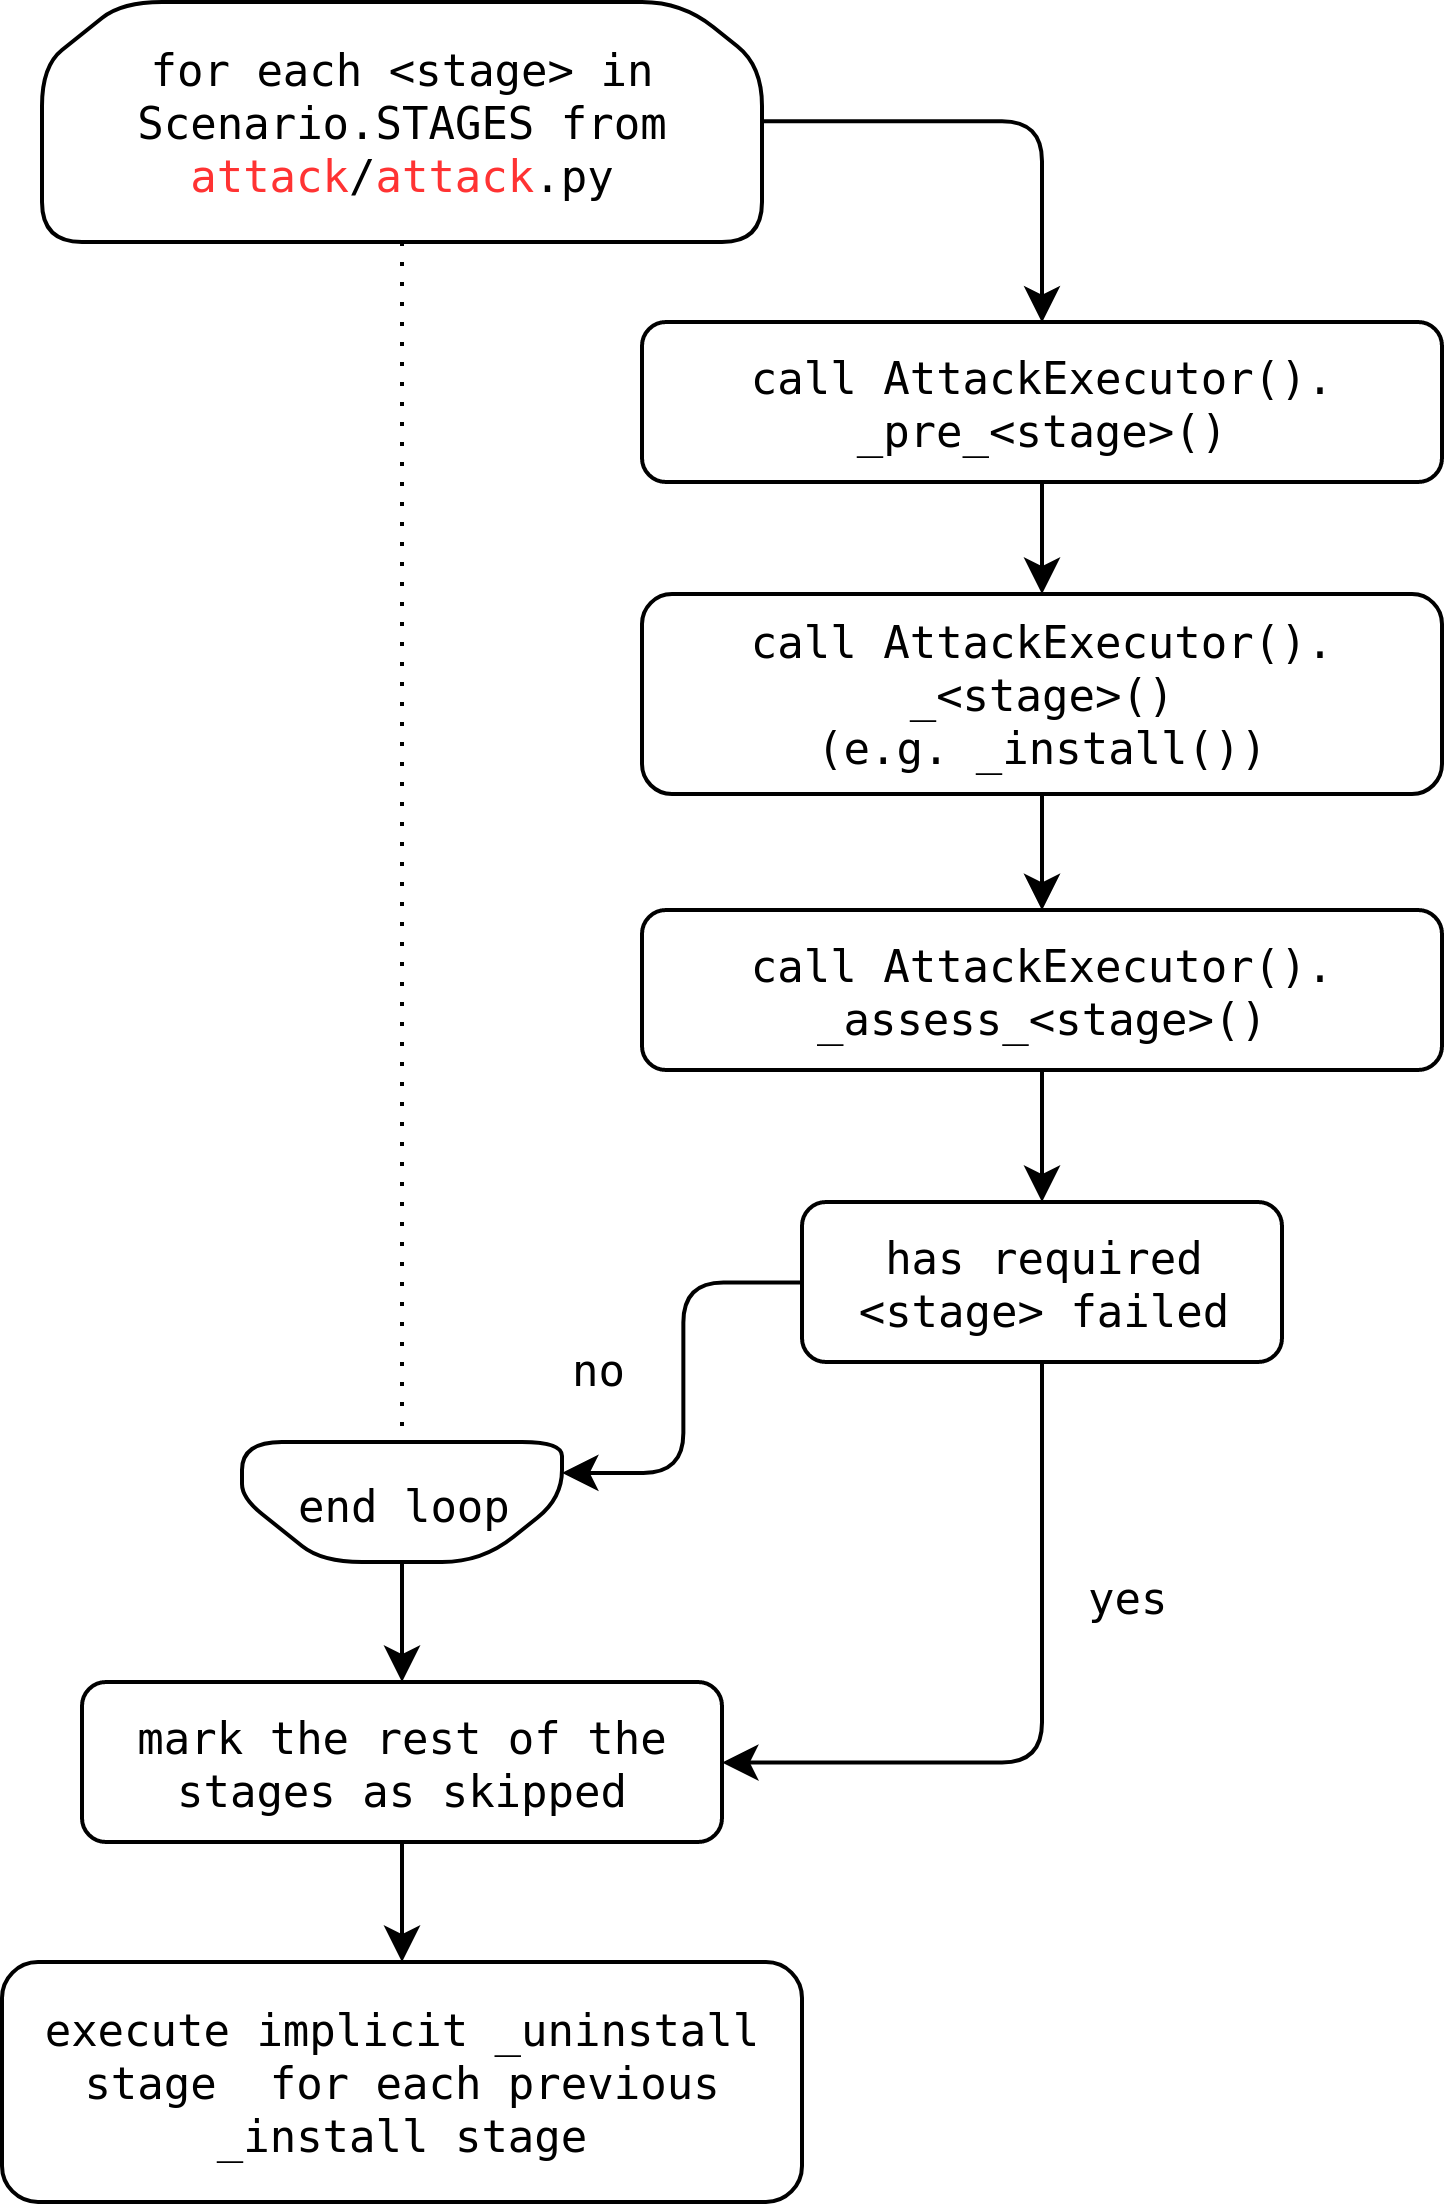
\includegraphics[width=0.7\textwidth]{src/diagrams/execute-scenario.png}
            \caption{Control flow graph explaining the order of execution of different stage methods.}
            \label{fig:execute-scenario}
        \end{figure}

            % \subsection{The common stages}\label{subsec:common-stages}
            %     As we mentioned in~\ref{subsec:executor:class} the common attack stages are (un)installation of CAP files and sending APDU commands. Internally those are implemented as methods on the \shortexecutorclass class. 

                % Due to the way JavaCard environment is build, it is only natural, that multiple attacks have similar structure --- installation, sending APDU commands and uninstallation. The JavaCard Vulnerability Scanner framework comes with those three stages already implemented, but the user of the application can easily extend it with their own (we will explain how to do so later). Internally as seen from the JavaCard Vulnerability Scanner framework point of view each stages is a Python function (or rather method, as it is a class funcion). As such it receives certain parameters and returns a value. Now we will go through the stages already implemented by JavaCard Vulnerability Scanner.

        % \subsubsection{install}
        %     As apparent from the name, this stage is used for installing packages and applets. This stage can install only one CAP file at a time, but can use this stage multiple times within one scenario. The parameters for this stage are listed in~\ref{fig:stage-install-params}.
            % \begin{figure}[h!]
            % \begin{enumerate}[align=left]
            %     \item[name] 
            %     \item[path]
            %     \item[comment]
            %     \item[optional]
            % \end{enumerate}
            % \end{figure}
            % "name": "install",
        %     "path": "build/{version}/com/se/vulns/javacard/vulns.new.cap",
        %     "comment": "The altered vulnerable applet",
        %     # install should be required by default
        %     "optional": False,
        % \subsubsection{send}
        % {
        %     "name": "send",
        %     "payload": "0x80 0x10 0x01 0x02	0x04	0x00 0x00 0xc0 0x00				0x7F",
        %     "comment": "read memory",
        %     "optional": True,
        % },
        % \subsubsection{uninstall}



    % Now that we have defined some terms we can look at some of them in greater detail.

            
    
    % TODO what with thiss
    % After discussing the ins and outs of the logical attack against the JavaCard platform we will explain the design of the testing tool \javus. Few key points need to be stressed. It is a prototype.
        % \subsection{Defining stages}
        % Now that we have means how to build and rebuild the attack during the runtime we can move on to defining the scenario and it's stages. The stages need to be defined in the module file \mintinline{python}{example_attack.py}.



    \subsubsection{Custom stage definition}\label{subsubsec:custom-stage}
    In case the default stages are not covering a particular step in the attack scenario we can add a custom stage. Let us call it \mintinline{python}{foobar}. Similarly to the default stages we will add the \mintinline{python}{foobar} stage to the \mintinline{python}{Scenario.STAGES} list. However, because it is a custom stage we need to also implement it. We must at least define the methods \mintinline{python}{_foobar}, that implements the main stage logic and \mintinline{python}{_assess_foobar}, which must accept the dictionary parameter \mintinline{python}{result} and populate its \mintinline{python}{"success"} key with either \mintinline{python}{True} or \mintinline{python}{False} value. We can also implemnent the \mintinline{python}{_pre_foobar} method and do any setup needed for the stage. All these methods are defined on the \attackexecutor class, that subclasses \shortexecutorclass (if it is not clear where to place this class see~\ref{subsec:executor:class}).



        All of the \mintinline{python}{"<key>": "<value>"} pairs except the \mintinline{python}{"name"} from the stage definition are passed as keyword arguments to the stage methods. Therefore the stage methods need to accept them (we can also make use of the \mintinline{python}{*args, **kwargs} Python syntax to accepts \textit{any} arguments). The example code is in the Appendix in listing~\ref{lst:new:stage}. The \mintinline{python}{AnalysisManager} will attempt to save the complete contents of \mintinline{python}{result} dictionary from the listing~\ref{lst:new:stage} to the database. However, only Python values, that can be encoded as BSON with Python \mintinline{python}{bson} module will be saved.

    \subsection{Registering the attack}
    As of now, the only way to add a new attack is to work in the structure of the Git project --- it's not possible to register an attack, that is outside of the project directory tree. Therefore, make sure, that the attack (in our case \texttt{example_attack}) files reside in the directory \filepath{javus/data/attacks/example_attack}.

    The last thing needed for the attack to be executed by the framework is to add a line to the file \filepath{javus/data/registry.ini}. This file follows a simple structure. Attacks are grouped by sections (e.g.\ the attacks from Security Explorations are in the section \mintinline[breaklines,breakbefore=E]{python}{[SECURITY EXPLORATIONS]}). The user picks an appropriate section or add a new one and add a new line entry saying \mintinline{ini}{example_attack = yes} (if the user wants to let the framework know about the attack, but disable it for now from the analysis set the value to \mintinline{ini}{no}). The user can verify, that the attack is registered by running \mintinline{bash}{javus list}. The user should see his attack in the output.

    \subsection{Validating the attack}
    To help the user with adding a new attack we have also implemented a \mintinline{python}{validate} sub command for the script \javus. \mintinline[breaklines]{python}{javus validate --attack <attack-name>} will validate the \texttt{<attack-name>}. Stage execution can not be easily validated, so the user should be careful.
    % is provided then only the \mintinline{bash}{<attack-name} attack is validated. However, not everything about the attack can be validated (e.g.\ saving custom results of custom stages) so the user might need to be cautious.




    \section{Invocation of \javus}\label{sec:invocation}
        \projectname has a several software dependencies (see the list Appendix in~\ref{subsec:3rd-party}) and it also needs the access to the hardware peripheral devices --- the smartcard readers. Due to those reasons, it is not so straightforward to run \javus. The testing tool is also required to be cross-platform --- execute at least on Linux and Windows. Therefore, we will take a moment now to explain, how to execute \javus in various environments. To avoid any confusion --- the testing tool operates on a physical JavaCard, which implies, that the user needs a smartcard reader and a JavaCard plugged in.

        \subsection{Native invocation on Unix platforms}\label{subsec:native-invocation}
        This tool was developed natively on Linux (Ubuntu 18.04). Invoking the framework on Linux is the easiest way how to perform the analysis, because we have a direct access to the smartcard readers (no matter if built-in or external ones). The downside of this approach is the need to install several software tools directly on the system. In order to bootstrap the Ubuntu environment the user can utilize the Bash script \mintinline{bash}{bin/bootstrap-ubuntu-18.04.sh}. It will install all the necessary software requirements. The details, along with a setup script are in the appendix. The bootstrap script can also be used from within a virtual environment (tested with VirtualBox v6.1.10), however, the user will need to make sure, that the smartcard readers are accessible inside the virtual environment . Once everything is set up correctly and a single JavaCard is inserted  into the reader the command \mintinline{bash}{pipenv run javus} can be invoked. Or if Pipenv is activated, \javus can be called directly, without any prefix.

        \subsection{Building a Docker image for Docker container}\label{subsec:dock-build}
        Nowadays, a popular solution to achieve cross-platformity is Docker.  It is a form of virtualization, where the main idea is to create the smallest possible environment (called container), that has all the necessary dependencies and run a script/binary within this container. To start the user needs to write a \mintinline{bash}{Dockerfile}, that contains directives, that specify the various dependencies. Using this file Docker can build an \textit{image}, which is sort of a blueprint. A running instance of a Docker image is then a Docker container. A \mintinline{bash}{Dockerfile} directives define various stages (those are useful to speed up the build process of a Docker image). Again, we need the access to the underlying smartcard readers. This obstacle defeats a bit the cross-platform feature of Docker, but we can overcome it. What we need to do, is to pass the smartcard readers into the Docker container allowing the framework to see them. Secondly, we will expose the port \mintinline{bash}{5000} for the viewer application, so that it is accessible outside of the container.

        % FIXME add to dockerhub?
        The Docker image for JavaCard Vulnerability Scanner is not available for download yet, but the user can build it locally. This requires Docker to be installed and then to run:
        \begin{minted}[fontsize=\footnotesize]{bash}
$ docker build --tag javus .
[...]
# or use the develpoment tool Invoke and run
$ inv dock
[...]
        \end{minted}

        As explained previously, making it so that the Docker container sees the smartcard readers requires different setup on Linux and Windows platforms.

        \subsection{Starting a Docker container on a Linux host}\label{subsec:inv-docker-unix}
        For Linux things are simpler. During the startup of the container we need to give the absolute paths to the USB devices. For the convenience of the user we have added a Bash script \mintinline{bash}{bin/javus-docker-unix}, that tries to find all the available smartcard readers and starts the \mintinline{bash}{javus-container} Docker container with the readers visible to the application inside.


        \subsection{Starting \javus inside a VirtualBox}\label{subsec:vb-invocation}
        In case the previous solutions do not work, there is one more option. It requires installing and setting up VirtualBox with Ubuntu 18.04 machine and then following the instruction in~\ref{subsec:native-invocation} (inside the Ubuntu virtual machine). As with previous solutions, the user needs to make sure, that the virtual environment \textit{sees} the smartcard readers. The process explained in steps:

        \begin{enumerate}
            \item install the newest version of VirtualBox (tested by the author on v6.1.10) and the corresponding version of the VirtualBox ExtensionPack,
            \item\label{enum:vb-ubuntu-iso} create a new Ubuntu 18.04 based virtual machine in VirtualBox,
            \item set up USB filters in VirtualBox to pass through the smartcard readers into the machine from~\ref{enum:vb-ubuntu-iso},
            \item use Git to clone the current version of JavaCard Vulnerability Scanner into the Ubuntu guest and bootstrap the environment as in~\ref{subsec:native-invocation}.
        \end{enumerate}

        This approach should work on any platform, that supports VirtualBox.

        \subsection{Starting a Docker container on a Windows host}
        The situation on Windows is more complicated. First of all, there are different versions of Docker~\cite{dockertoolbox, dockerforwindows}, that can be installed on Windows machine and, only Docker Toolbox~\cite{dockertoolbox} allowed to pass the smartcard readers. Together with Docker the user should get also VirtualBox and \mintinline{bash}{docker-machine} already as one of the virtual machines. The user will need to follow similar steps from the previous subsection \label{subsec:vb-invocation} of setting up the VirtualBox, so that the \mintinline{bash}{docker-machine} has access to the smartcard readers.

        Since there are multiple ways of invoking the command line utility \javus (all of the presented solutions are in some sense just complicated wrappers, that at the end invoke \javus) we will unify the invocation of JavaCard Vulnerability Scanner in the examples and simply write \javus, the reader is expected to substitute this command in case he is invoking the utility in a different way (e.g. using \mintinline{bash}{javus-docker-unix}).


% component was required, but the applets allows installation with it missing
% FIXME it worked on few cards - check if the components are required or not in the particular specification


\subsection{Discovering discrepencies between off card and on-card BCV}\label{subsec:onofffuzzing}

    \cite{ossfuzz} shows, how fuzzing technique can be utilized for testing the robustnes and security of applications. We have not seen this technique used in the area of Java Card platform. Fuzz testing is based on multitude of random or semi-random test inputs. For real JavaCards it is what to fuzz, because if we just tried to flood the JavaCard with APDUs we would probably quicky block or at least mute the card.
        One possible fuzzing scenario is the following, we will start with a working CAP file, then create a fuzzed version of that file. If this new CAP file fails the off-card verification process, we will attempt to install it on a real card. If the card accepts it, it means, that the on-card bytecode verifier is not \textit{aligned} with the off-card one. On the next few lines the reader can see pseudo code of this fuzzing technique:

\begin{minted}[linenos]{text}
 generate a valid CAP file valid.cap
 use fuzz valid.cap to generate fuzzed.cap
 verify fuzzed.cap with off-card
 if verification succeeds:
    continue to line 1
 else:
    try to install fuzzed.cap onto a target JavaCard
    if the installation fails:
        continue to line 1
    else: 
        save the file fuzzed.cap as witness.cap
\end{minted}
We have yet to fully explore this technique, but within minutes of trying it we had first few \texttt{witness.cap} files, for which the off-card verifier gave an error, however a card allowed the installation. We have used~\cite{radamsa} for fuzzing.



    % \section{Final notes about JavaCard Vulnerability Scanner}
    %         Since this project consists of several different command line utilities and features, that cover the development of this project and also its usage, we provide a list explaining shortly each of them to help the reader navigate in the tools.


%                 \begin{enumerate}[align=left]
%                     \item[\texttt{test}\label{enum:inv-test}] tests the project by executing the complete Python test-suite (the underlying test runner is Pytest),
%                     \item[\texttt{check}] executes checks on the live environment. In contrast to testing, checking uses the live environment. For example, it checks, that the necessary dependencies, like Ant, are installed,
%                         \label{enum:inv-check}
%                     \item[\texttt{develop}] sets up the development in such a way, that the subsequent edits are immediately reflected in the \javus utility (speeds up the development, because the tool does not need to be installed after every edit),
%                     \item[\texttt{dock}] builds a fresh Docker image from the project,
%                     \item[\texttt{docs}] builds the documentation for the project.
%                 \end{enumerate}

%             Each Invoke task is accessible from the command line by executing \texttt{inv[oke] <task-name>} from the command line. The \texttt{<task-name>} is a placeholder, so for example to execute the test suite one has to call \texttt{inv test}.

%             \subsection{The \javusdev utility}\label{subsubsec:javusdev}


